% ============================================================
% ［架空の記入例・提出不可］研究設定，データ，数値および結果はすべて架空である．
% 通常のchapters/05-experiments.texには自動で読み込まれない．
% ============================================================
\chapter{実験・評価}

\begin{center}
  \UsamiFictionalExampleNotice
\end{center}

\section{データと評価手順}

説明用に設定した架空の室内動画12系列，2,400フレームを用いた．同じ撮影系列の隣接フレームが異なる分割へ混入しないよう，動画系列単位で学習4系列，検証4系列，評価4系列へ分けた．評価系列には，通常照明，低照度，動きぼけの3条件を含めた．図\ref{fig:experiment-design}に示すように，検証系列で閾値を決定した後，評価系列ではパラメータを固定して指標を集計した．

\begin{figure}[tb]
  \centering
  % SVG原稿とPDF版をexamples/figures/へ同梱している．
  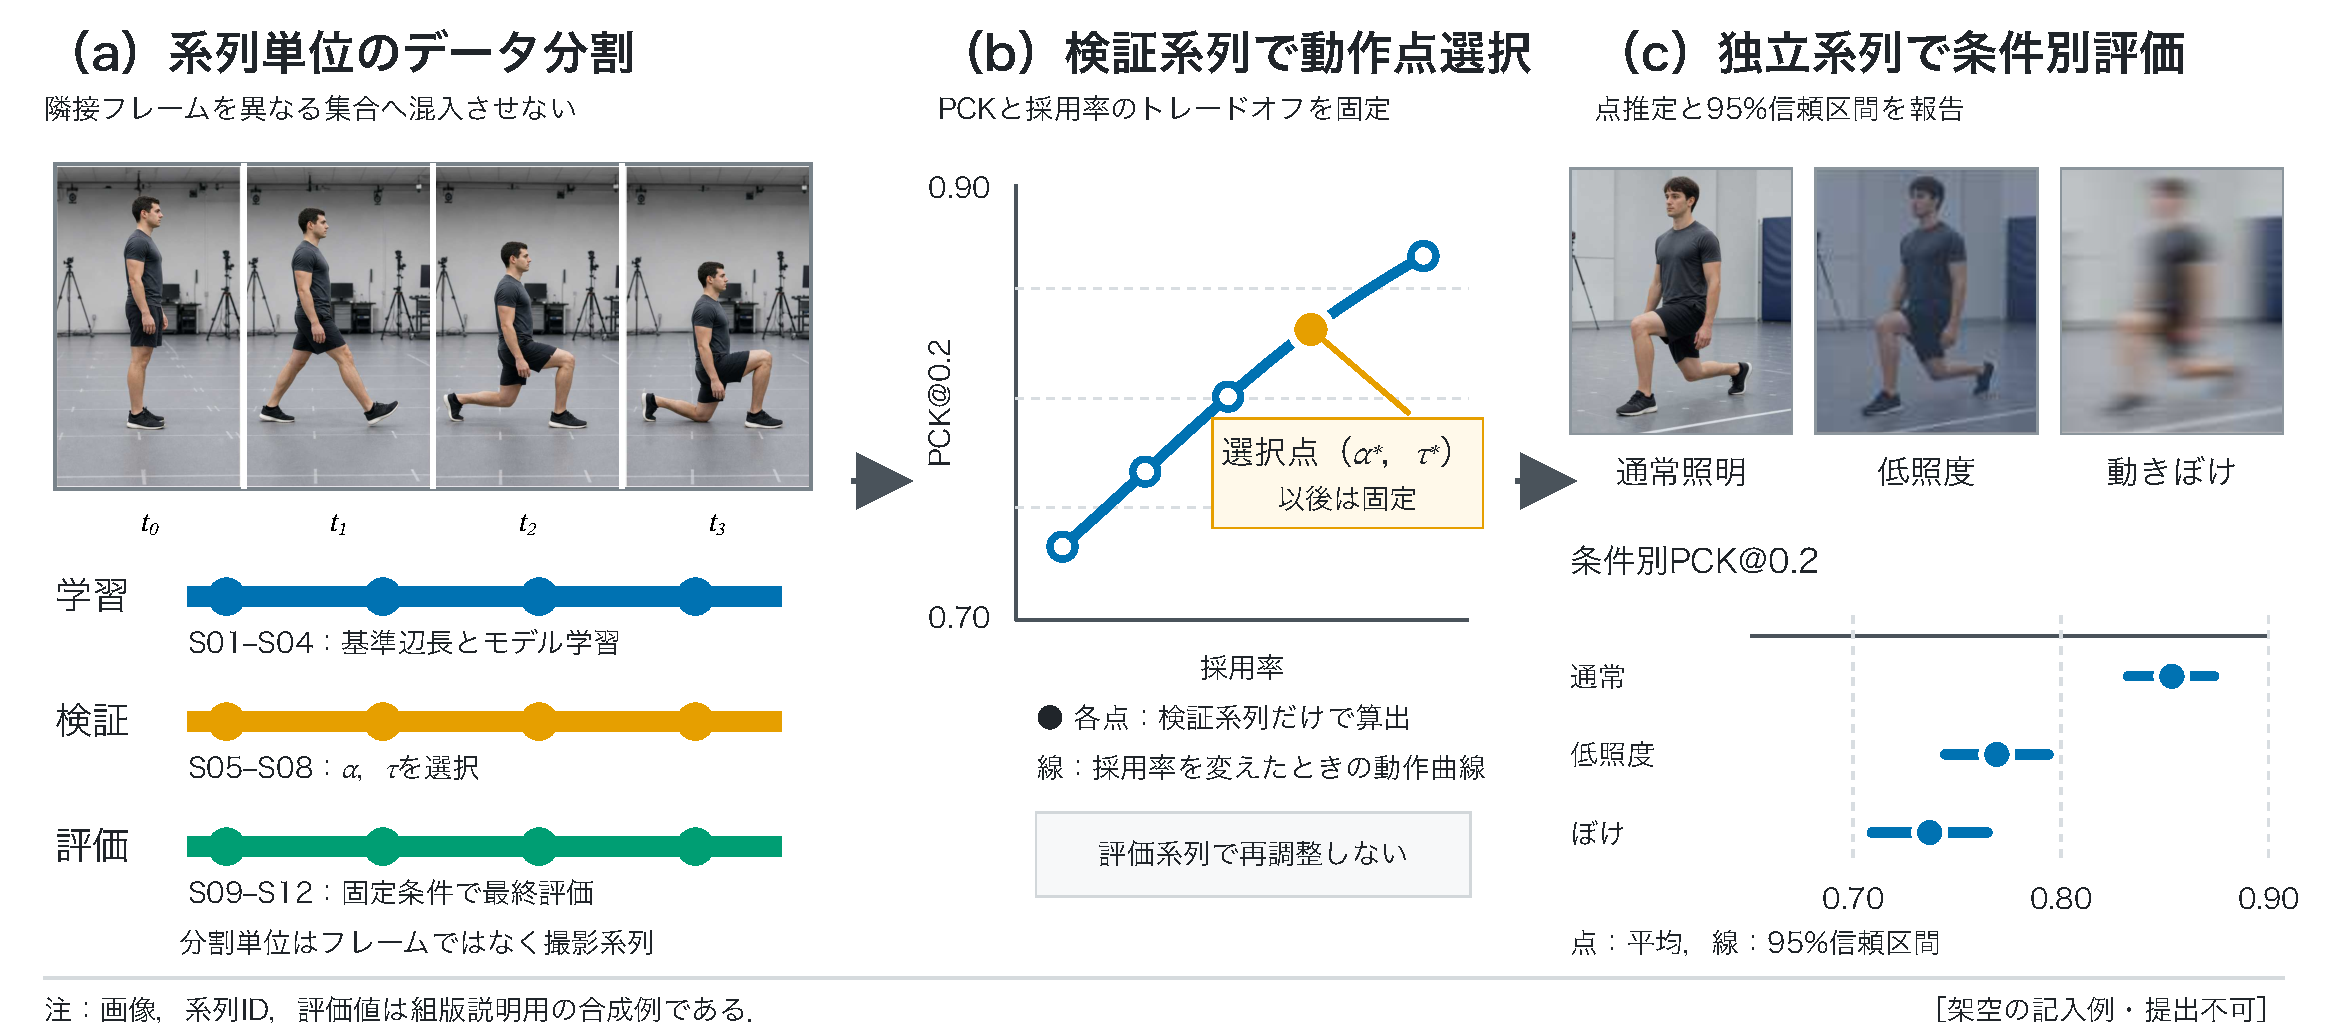
\includegraphics[width=\textwidth]{examples/figures/experiment-design.pdf}
  \caption{データ分割と評価手順．系列間の情報漏洩を避けて評価する}
  \label{fig:experiment-design}
\end{figure}

\section{比較条件と評価指標}

比較条件は，骨格を除外しない条件，平均関節信頼度だけで除外する条件，式\eqref{eq:method-quality-score}の提案スコアで除外する条件の3つとした．採用した骨格の関節位置精度をPCK@0.2で評価し，これと併せて全検出骨格に対する採用率を報告した．PCKのみを最大化すると難しいフレームを多数除外できるため，採用率を必ず同時に確認する．

\section{結果}

低照度条件の架空結果を表\ref{tab:experiment-results}に示す．提案スコアは，除外なしと比べて採用骨格のPCK@0.2が8.9ポイント高かった一方，採用率は18.3ポイント低下した．平均関節信頼度と比べると，PCK@0.2は3.9ポイント高く，採用率は4.7ポイント低かった．これは，骨格辺長の項が信頼度だけでは除外できない構造的な誤推定にも反応した可能性を示す．

\begin{table}[tb]
  \centering
  \caption{低照度条件における誤推定骨格除外の結果（架空値）}
  \label{tab:experiment-results}
  \begin{tabularx}{0.82\textwidth}{@{}Xcc@{}}
    \toprule
    除外方法 & PCK@0.2［\%］ & 採用率［\%］ \\
    \midrule
    なし & 73.1 & 100.0 \\
    平均関節信頼度 & 78.2 & 86.4 \\
    提案スコア & \textbf{82.1} & 81.7 \\
    \bottomrule
  \end{tabularx}
\end{table}

\section{考察}

表\ref{tab:experiment-results}は，提案スコアが低精度骨格を優先して除外した可能性を示すが，姿勢推定器自体の改善を意味しない．誤除外，見逃し，採用率および後段性能を併せて閾値を選ぶ．
